\chapter{Mengenal Python dan Anaconda}
Tujuan pembelajaran pada pertemuan pertama antara lain:
\begin{enumerate}
\item
Mengerti sejarah python, perkembangan dan penggunaan python di perusahaan
\item
Memahami tahapan instalasi python dan anaconda
\item
Memahami cara penggunaan spyder
\end{enumerate}
Tugas dengan cara dikumpulkan dengan pull request ke github dengan menggunakan format latex pada repo yang dibuat oleh asisten IRC.

\section{Teori}
Praktek teori penunjang yang dikerjakan :
\begin{enumerate}
\item
Buat Resume Sejarah Python, perbedaan python 2 dan 3, dengan bahasa yang mudah dipahami dan dimengerti. Buatan sendiri bebas plagiat(10)
\item
Buat Resume Implementasi dan penggunaan Python di perusahaan dunia, bahasa yang mudah dipahami(10)
\end{enumerate}

\section{Instalasi}
Melakukan instalasi python dan anaconda versi 3 serta uji coba spyder. Dengan menggunakan bahasa yang mudah dimengerti dan bebas plagiat. 
Dan wajib skrinsut dari komputer sendiri.
\begin{enumerate}
\item
Instalasi python 3 (5)
\item
instalasi pip(5)
\item
cara setting environment (5)
\item
mencoba entrepreter/cli melakui terminal atau cmd windows(5)
\item 
Menjalankan dan mengupdate anaconda dan spyder(5)
\item
Cara menjalankan Script hello word di spyder(5)
\item
Cara menjalankan Script otomatis login aplikasi akademik dengan library selenium dan inputan user(5)
\item
Cara pemakaian variable explorer di spyder(5)
\end{enumerate}


\section{Identasi}
Membuat file main.py dan mengisinya dengan script contoh python penggunaan selenium(minimal 20 baris) yang melibatkan inputan user, kemudian mencoba untuk mengatasi error identasi.
\begin{enumerate}
	\item
Penjelasan Identasi (10)
	\item
jenis jenis error identasi yang didapat(10)
\item
cara membaca error(10)
\item 
cara menangani errornya(10)
\end{enumerate}

\section{Presentasi Tugas}
Pada pertemuan ini, diadakan tiga penilaiain yaitu penilaian untuk tugas mingguan dengan nilai maksimal 100. Kemudian dalam satu minggu kedepan maksimal sebelum waktu mata kuliah. Ada presentasi kematerian dengan nilai presentasi yang terpisah masing-masing 100. Dan nilai terpisah untuk tutorial dari jawaban tugas di YouTube.Jadi ada tiga komponen penilaiain pada pertemuan ini yaitu :
\begin{enumerate}
	\item tugas minggu hari ini dan besok (maks 100). pada chapter ini
	\item presentasi csv (maks 100). Mempraktekkan kode python dan menjelaskan cara kerjanya.
	\item pembuatan video tutorial youtube tentang tutorial dari jawaban tugas.(nilai maks 100)
\end{enumerate}
Waktu presentasi pada jam kerja di IRC. Kriteria penilaian presentasi sangat sederhana, presenter akan ditanyai 20(10 pertanyaan program, 10 pertanyaan teori) pertanyaan tentang pemahamannya menggunakan python dan program agan dibuat error hingga presenter bisa menyelesaikan errornya. jika presenter tidak bisa menjawab satu pertanyaan asisten maka nilai nol. Jika semua pertanyaan bisa dijawab maka nilai 100. Presentasi bisa diulang apabila gagal, sampai bisa mendapatkan nilai 100 dalam waktu satu minggu kedepan.
\par
\textbf{JAWABAN CHAPTER 1}
\par
\textbf{1.1 Teori}
\begin{enumerate}
    \item Python dibuat pertama kali oleh Guido Van Rossum berlokasi di  Centrum Wiskunde and Informatica (CWI) Belanda pada tahun 1990-an. Bahasa pemrograman Python terinspirasi dari bahasa pemrograman ABC hingga sekarang.
    \par
    Guido masih menjadi orang utama dalam pengembangan Python. Meskipun begitu dikaarenakan Python bersifat open source maka banyak orang juga ikut berkontribusi dalam mengembangkannya.
    \par
    Di tahun 1995, Guido melanjutkan pembuatan Python di Corporation for National Research Initiative (CNRI) di Virginia Amerika, di mana dia merilis beberapa versi dari Python.
    \par
    Pada Mei 2000, Guido dan tim Python pindah ke BeOpen.com dan membentuk tim BeOpen PythonLabs. Di bulan Oktober pada tahun yang sama, tim Python pindah ke Digital Creation (sekarang menjadi Perusahaan Zope). Pada tahun 2001, dibentuklah Organisasi Python yaitu Python Software Foundation (PSF). PSF merupakan organisasi nirlaba yang dibuat khusus untuk semua hal yang berkaitan dengan hak intelektual Python. Perusahaan Zope menjadi anggota sponsor dari PSF.
    \par
    Semua versi Python yang dirilis bersifat open source. Dalam sejarahnya, hampir semua rilis Python menggunakan lisensi GFL-compatible.
    \par
    Versi python ini yang populer saat ini adalah python versi 3.5.x dan versi 2.7.x . Tanda “x” ini merupakan angka sub versi yang mungkin dapat berubah seiring perkembangan dari pihak pengembangnya. Namun orang - orang biasa menyingkat versinya menjadi python versi 2 dan python versi 3. Hal tersebut akan memudahkan kita untuk menyebutnya.
    \par
    \item Contoh implementasi Python pada perusahaan dunia salah satunya adalah Youtube. Python dipilih perusahaan ini dalam menganalisis data. Dapat kita lihat pada bagaimana cara Youtube merekomendasikan video. Contohnya jika anda sering mendengarkan dan melihat video musik pada platform Youtube maka Youtube dengan otomatis merekomendasikan apa yang sering anda cari di Youtube.
    \par
    Youtube memanfaatkan Python untuk analisis. Mereka memanfaatkan Luigi, yaitu salah satu modul dari Python, yang disinkronisasi dengan Hadoop, sebuah framework berbasis Java yang dapat melakukan pemrosesan data dengan ukuran sangat besar.
\end{enumerate}

\textbf{1.2 Instalasi}
\begin{enumerate}
\item Penginstalan Python 3.7

    \begin{itemize}
        \item Pertama jalankan instalasi dengan cara run administrator (Figure 1.1)
\item Klik kolom add Python 3.7 to PATH lalu klik Install Now (Figure 1.2)
\item Tunggu hingga prosesnya selesai (Figure 1.3)
\item Tunggu hingga prosesnya selesai (Figure 1.4)

    \begin{figure} [ht]
    \centering
    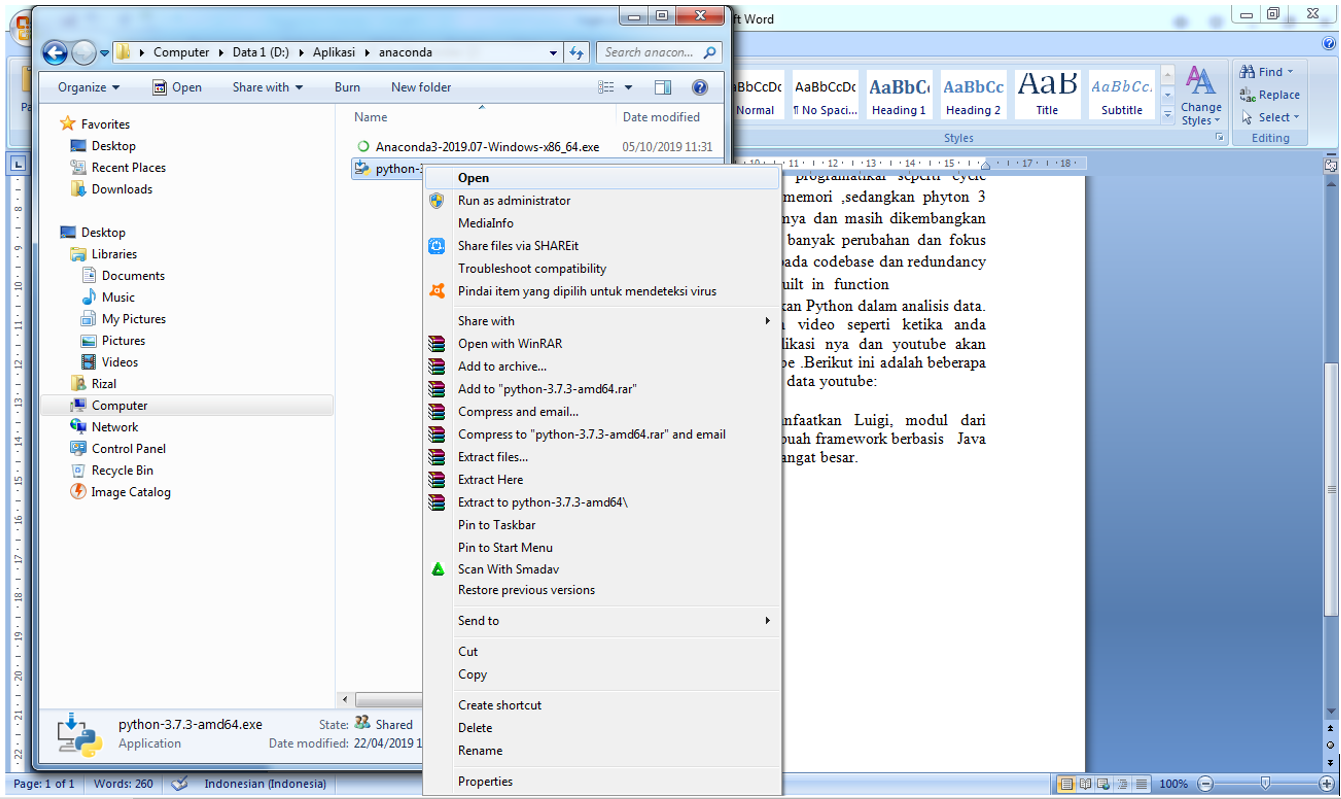
\includegraphics[scale=0.5]{figures/RA.PNG}
    \caption{Tahap pertama penginstalan Python}
\end{figure}

    \begin{figure} [ht]
    \centering
    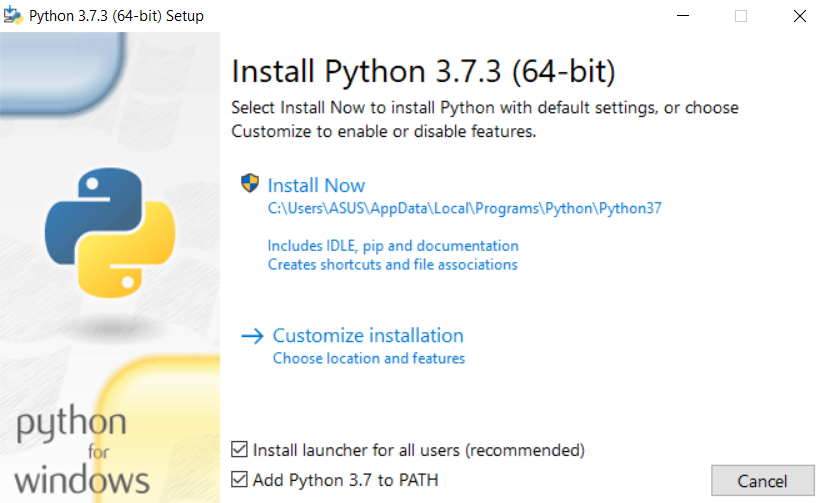
\includegraphics[scale=0.5]{figures/SS1.png}
    \caption{Tahap kedua penginstalan Python}
\end{figure}

    \begin{figure} [ht]
    \centering
    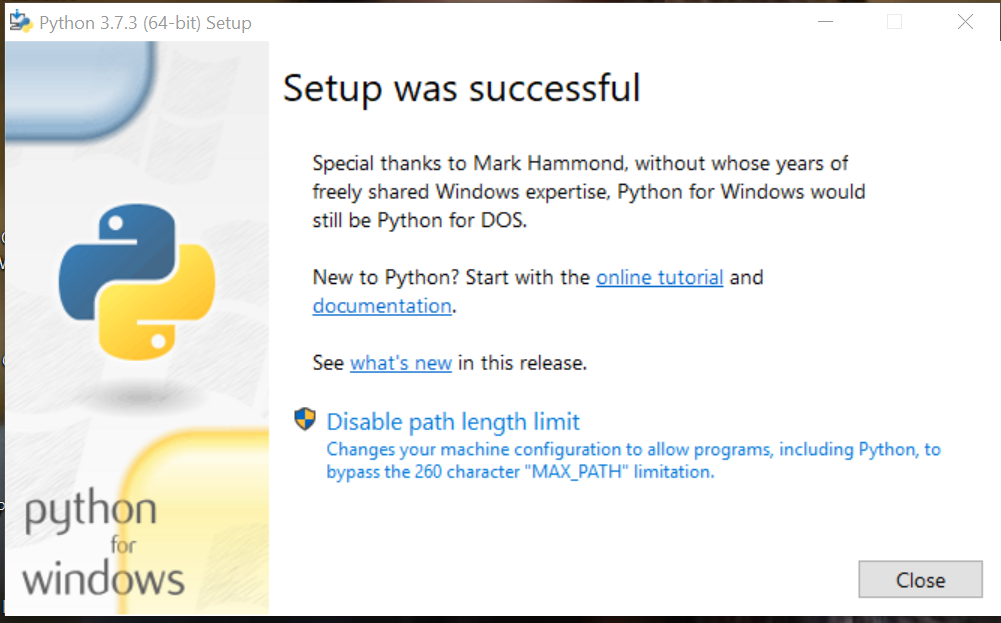
\includegraphics[scale=0.5]{figures/SS2.PNG}
    \caption{Tahap ketiga penginstalan Python}
\end{figure}

    \begin{figure} [ht]
    \centering
    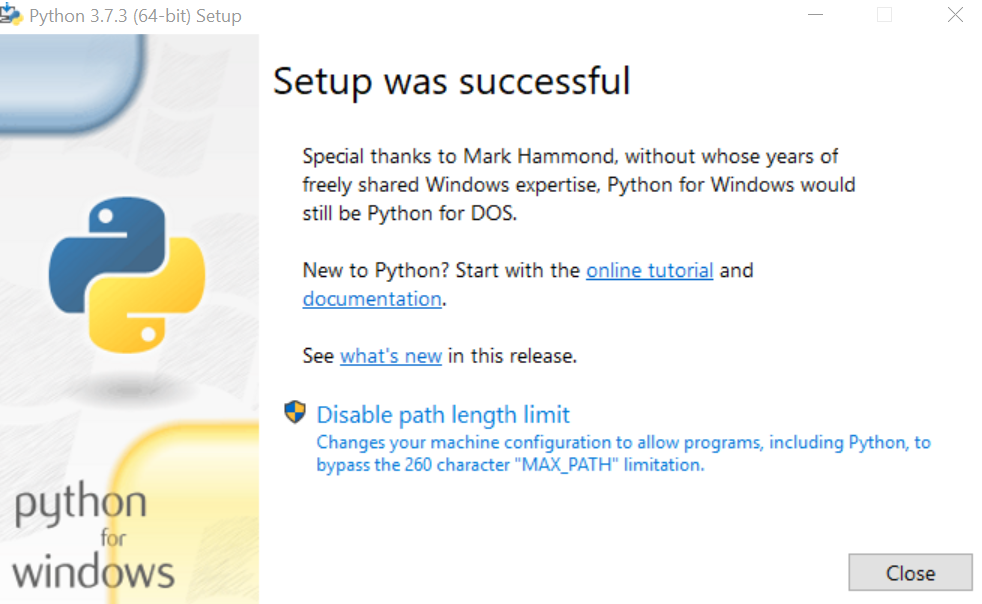
\includegraphics[scale=0.5]{figures/SS3.png}
    \caption{Tahap keempat penginstalan Python}
\end{figure}
    \end{itemize}


\item Penginstalan pip
   
\begin{itemize} 
\item Buka CDM(Command Prompt) melalui Start atau dengan cara tekan Windows+R secara bersamaan di keyboard (Figure 1.5)
    \begin{figure} [!htbp]
    \centering
    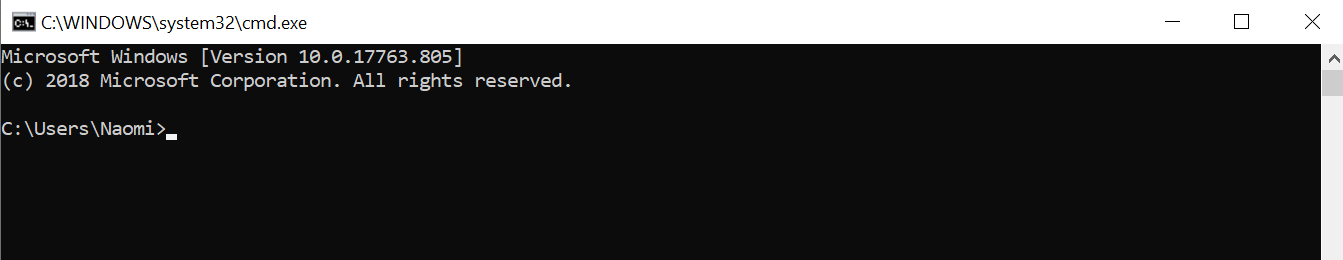
\includegraphics[scale=0.4]{figures/p1.png}
    \caption{Tahap pertama penginstall pip}
\end{figure}

\item Kemudian ketik “pip --version” pada CMD, lalu enter. Maka akan muncul seperti pada gambar (Figure 1.6)
    \begin{figure} [!htbp]
    \centering
    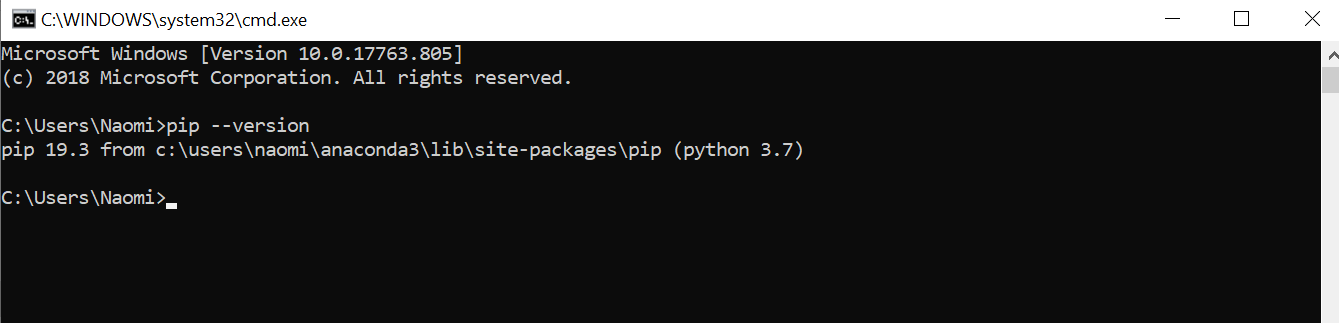
\includegraphics[scale=0.4]{figures/p2.png}
    \caption{Tahap kedua penginstall pip}
\end{figure}

\item Lalu ketik “python –m pip install –U pip” (Figure 1.7)
    \begin{figure} [!htbp]
    \centering
    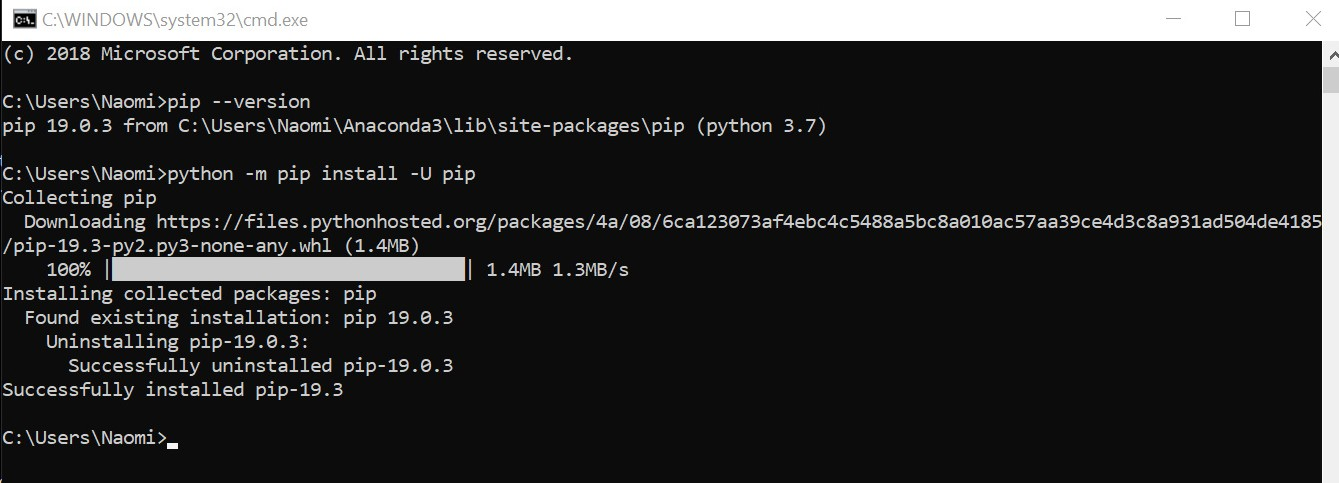
\includegraphics[scale=0.4]{figures/p3.jpg}
    \caption{Tahap ketiga penginstall pip}
\end{figure}
\item Pip install Python selesai.
\end{itemize}

\item Cara setting environment
\begin{itemize}
\item Pertama buka Anaconda Navigator. (Figure 1.8)
\item Lalu klik Environment (Figure 1.9)
\item lalu klik centang hijau yang ada di sebelah kiri (Figure 1.10)
\item Lalu klik versi yang paling terbaru. (Figure 1.11)
\item Kemudian Apply. (Figure 1.12)
\item Klik Apply (Figure 1.13)

    \begin{figure} [!htbp]
    \centering
    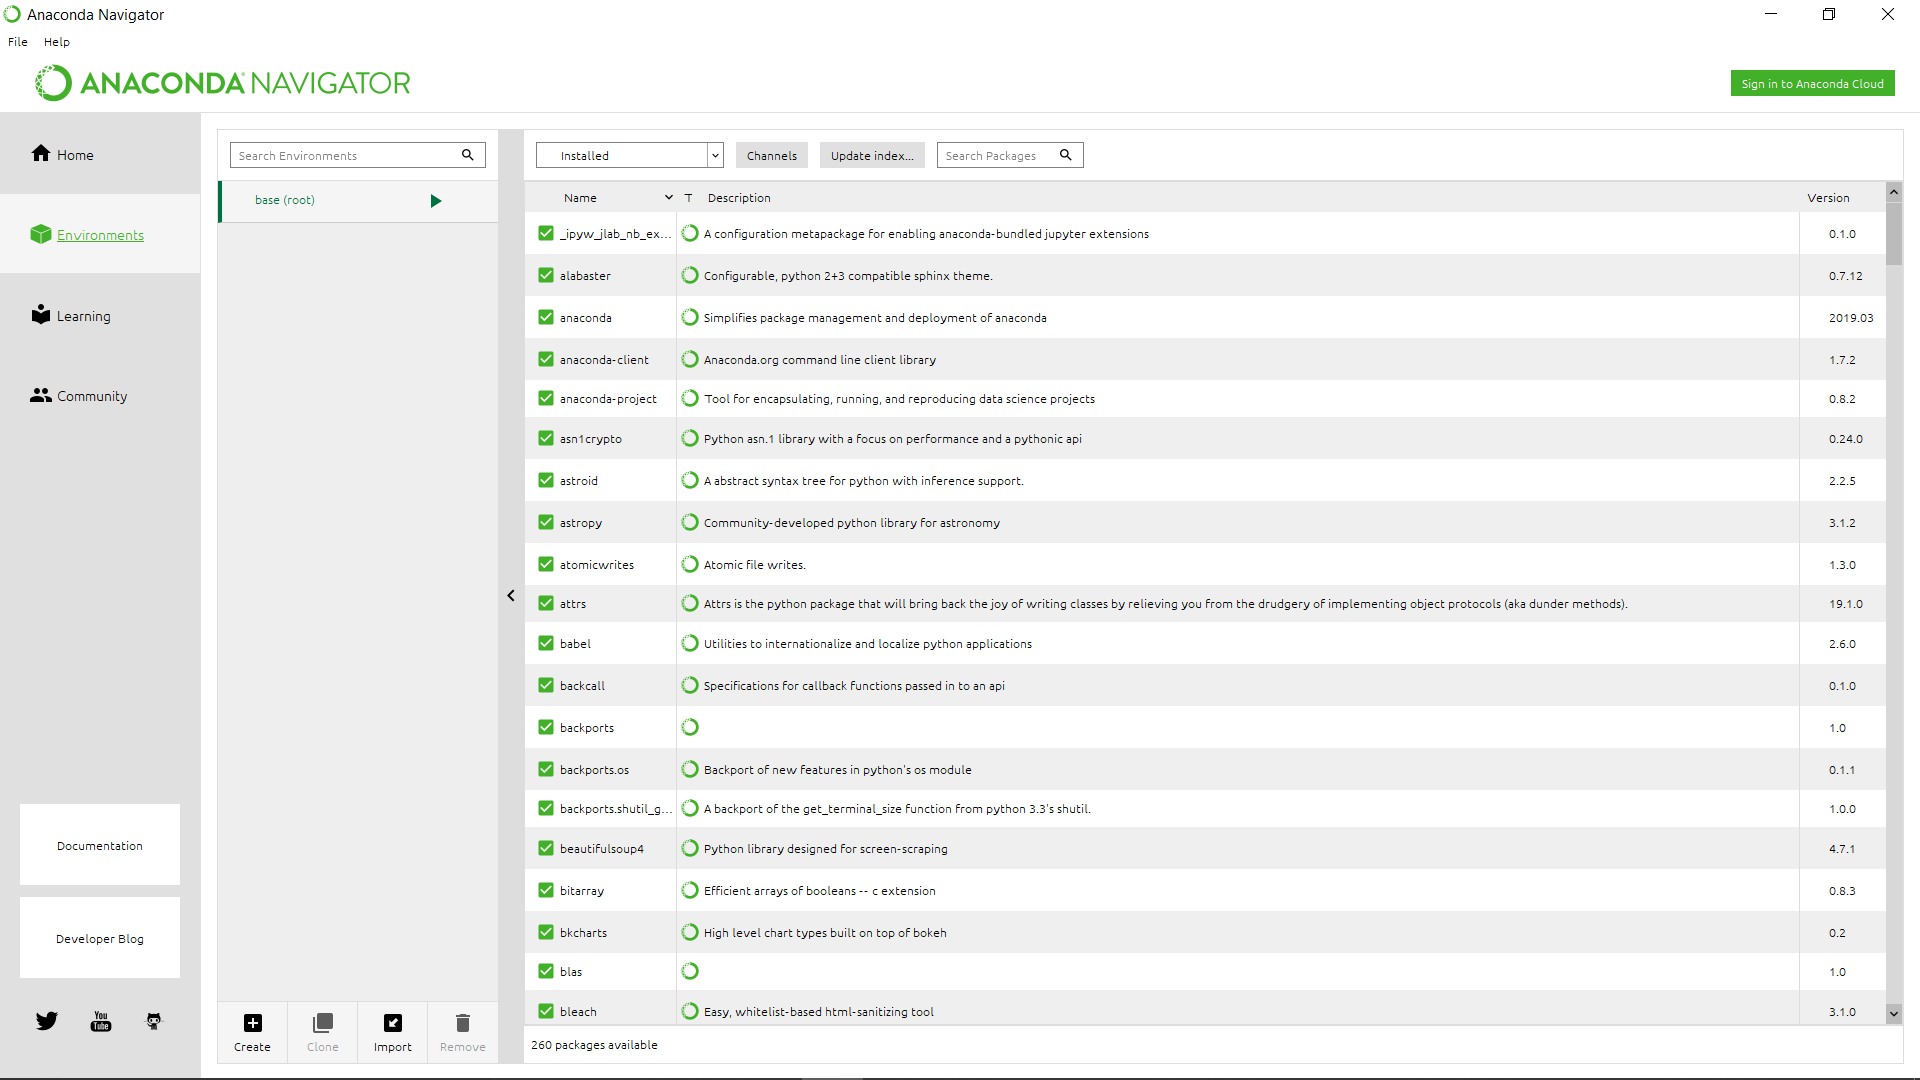
\includegraphics[scale=0.2]{figures/A3.png}
    \caption{Tahap pertama setting environment}
\end{figure}

    \begin{figure} [!htbp]
    \centering
    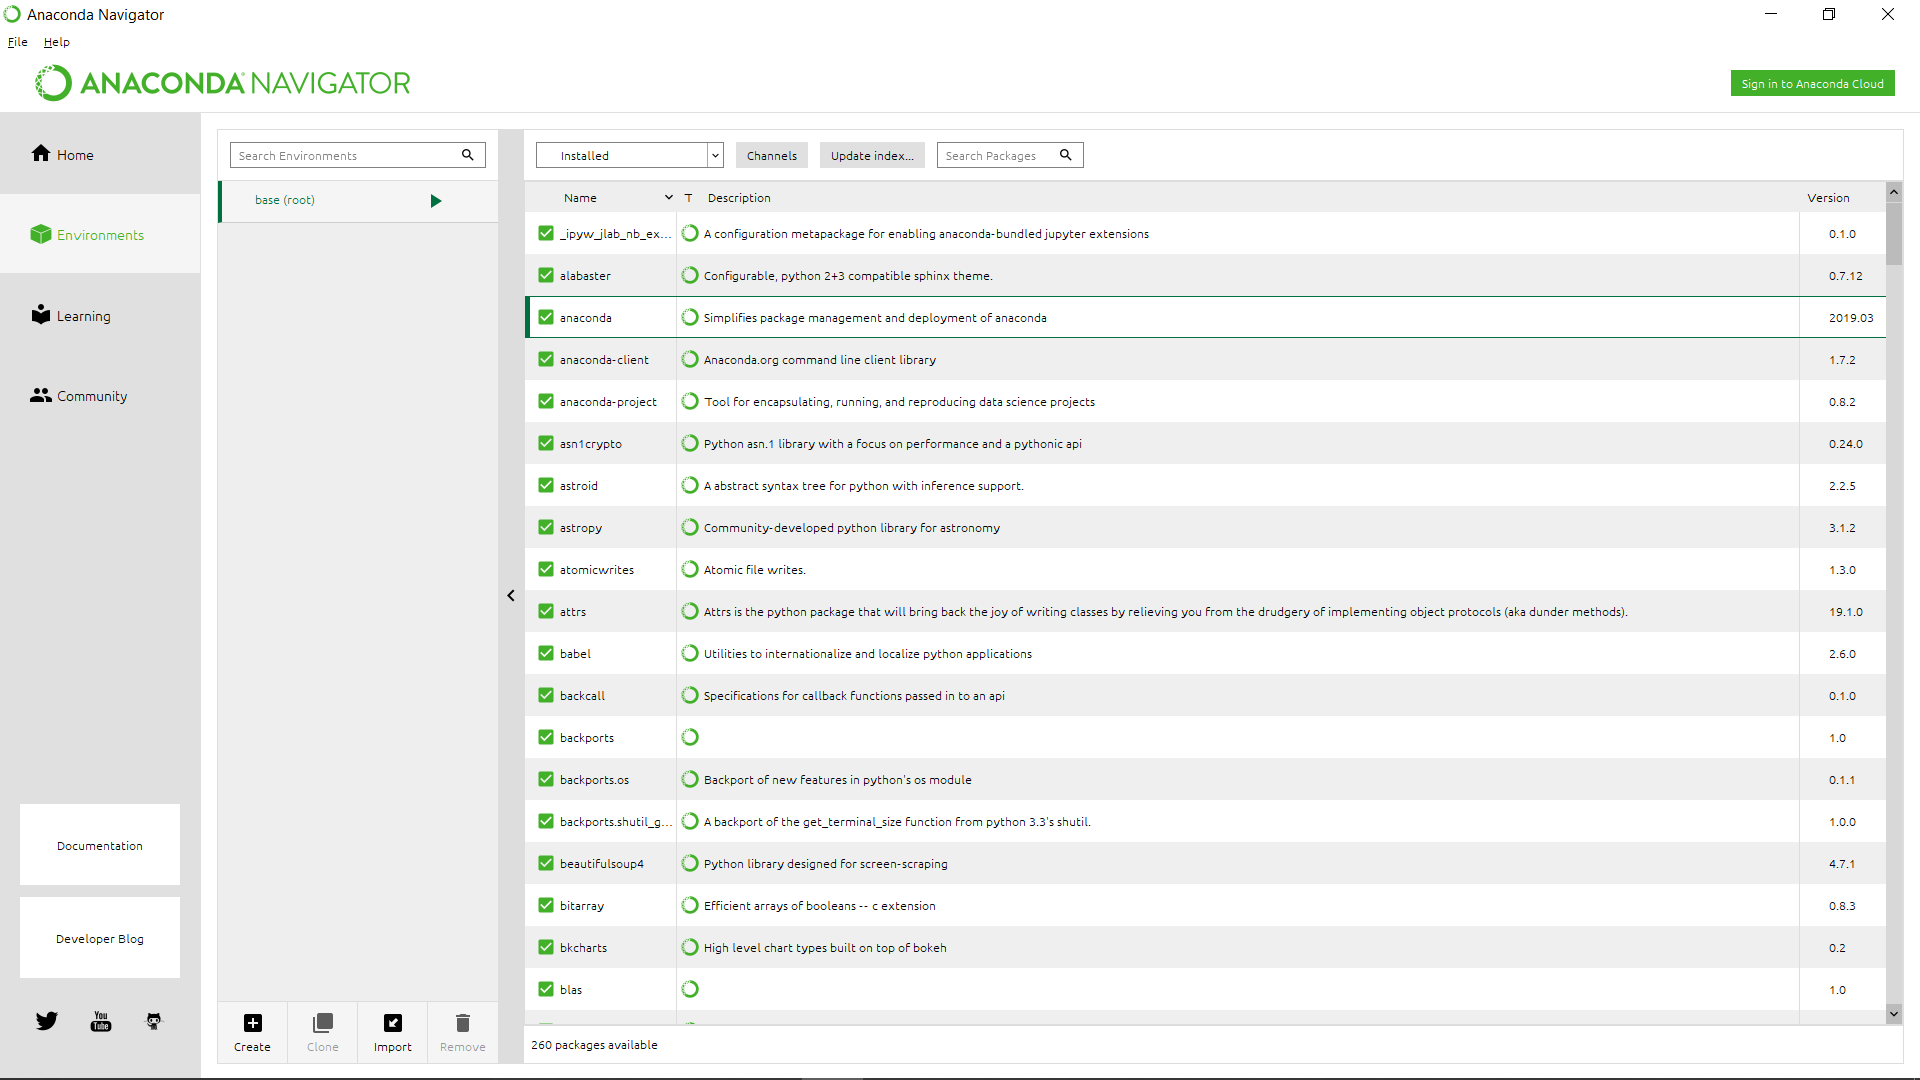
\includegraphics[scale=0.2]{figures/A4.png}
    \caption{Tahap kedua setting environment}
\end{figure}

    \begin{figure} [!htbp]
    \centering
    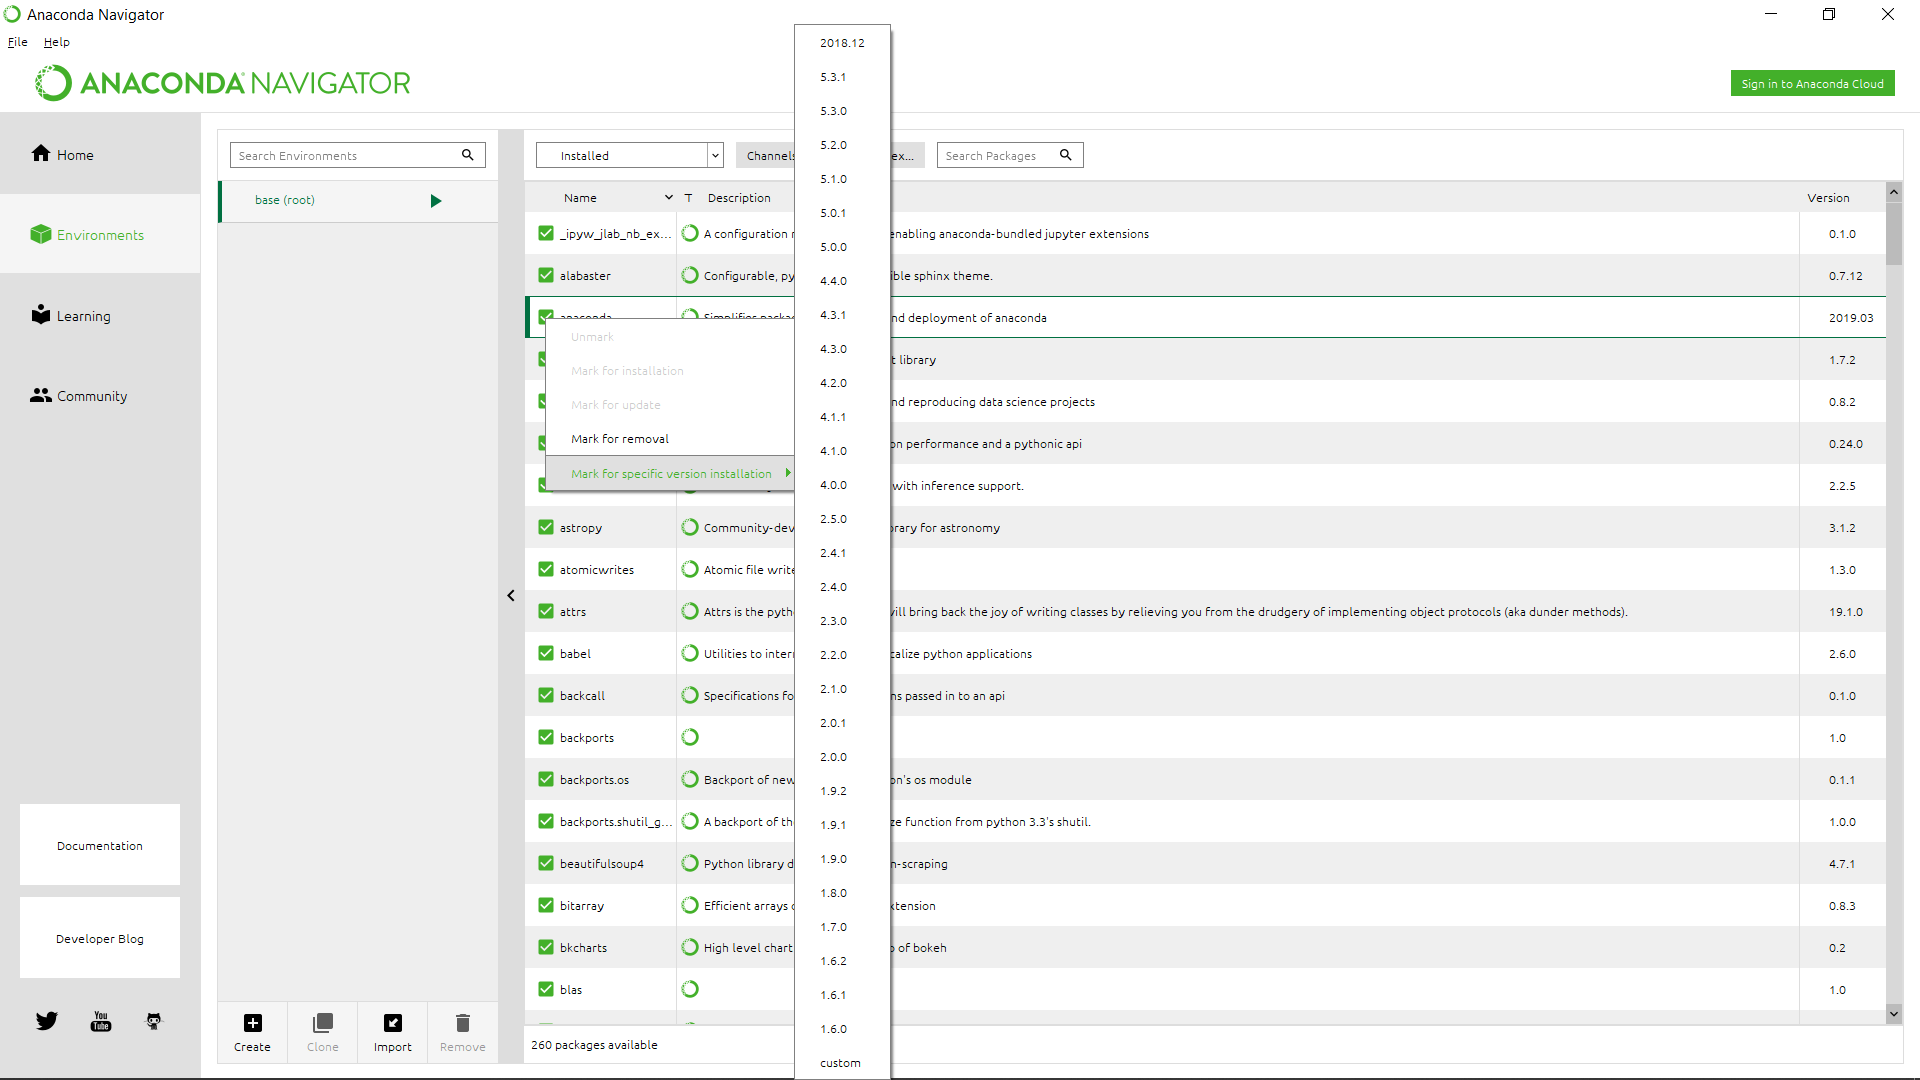
\includegraphics[scale=0.2]{figures/A5.png}
    \caption{Tahap ketiga setting environment}
\end{figure}

    \begin{figure} [!htbp]
    \centering
    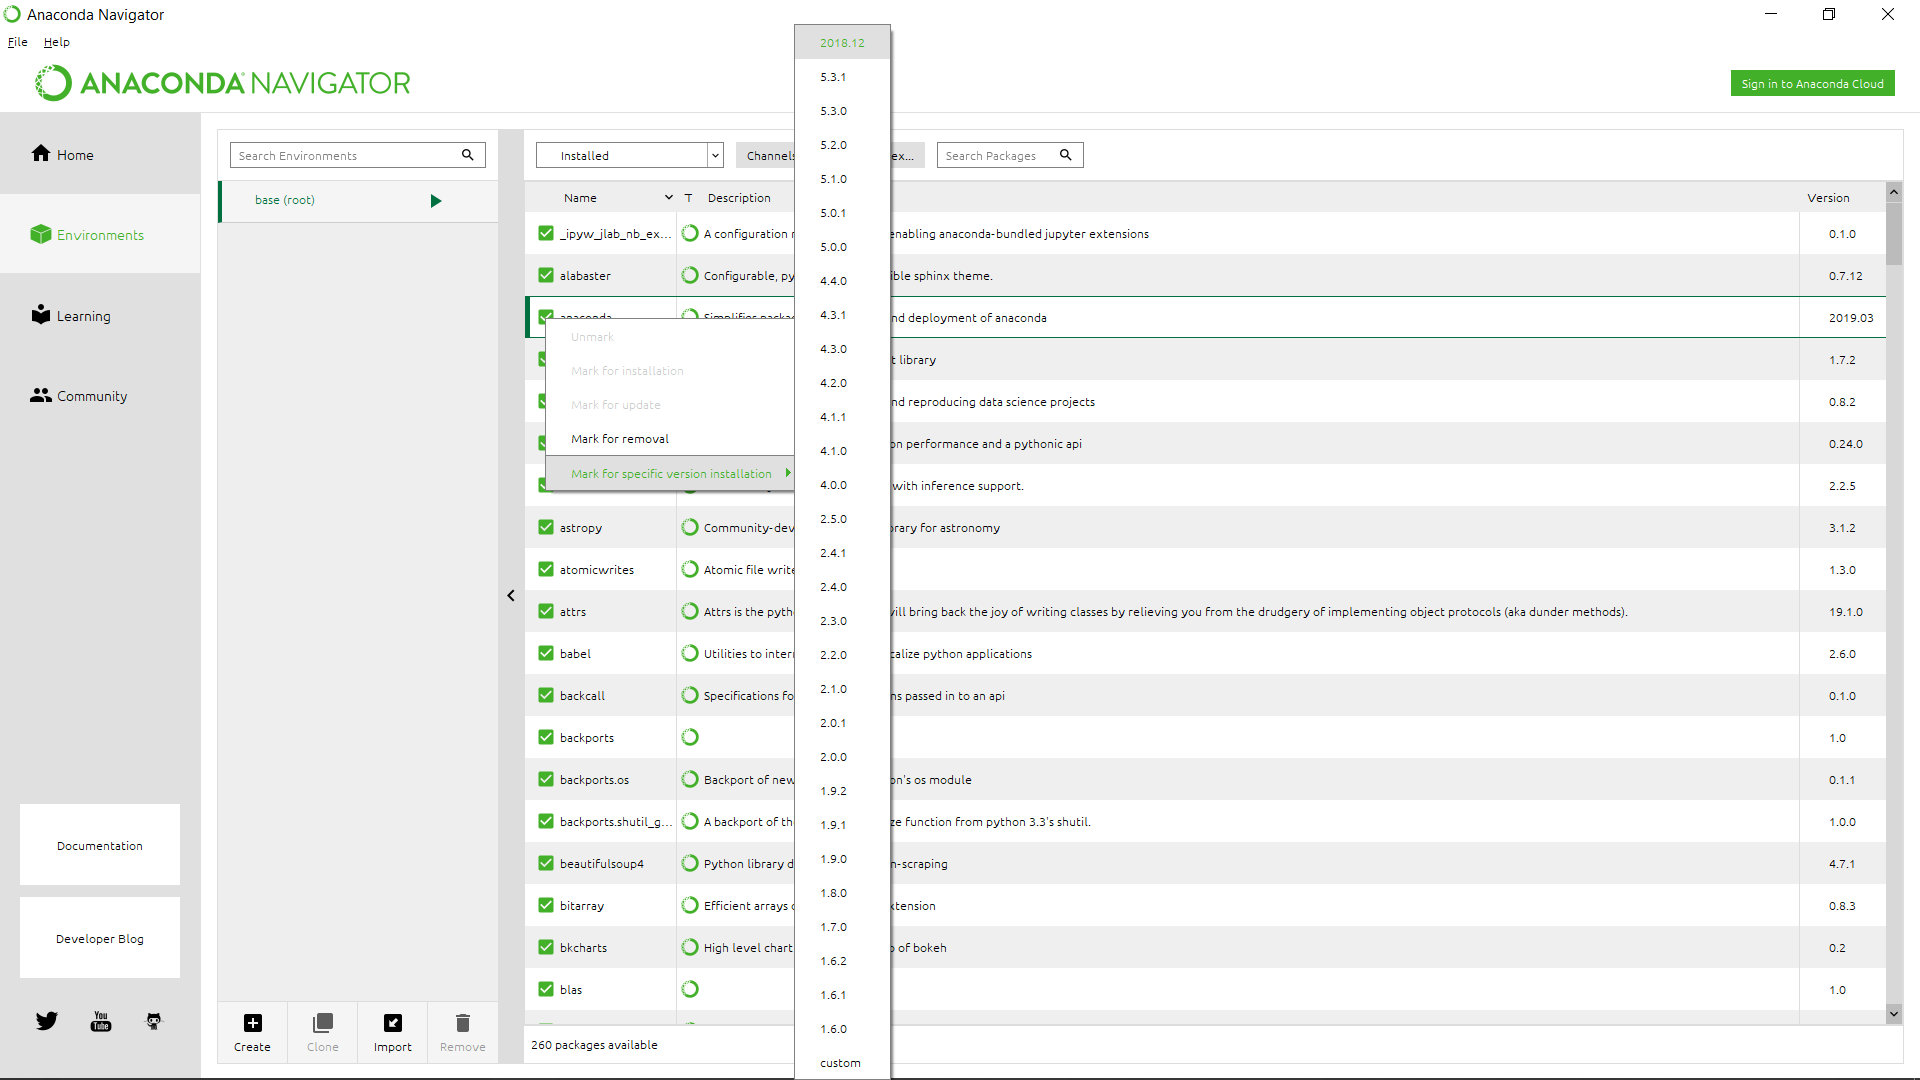
\includegraphics[scale=0.2]{figures/A6.png}
    \caption{Tahap keempat setting environment}
\end{figure}

    \begin{figure} [!htbp]
    \centering
    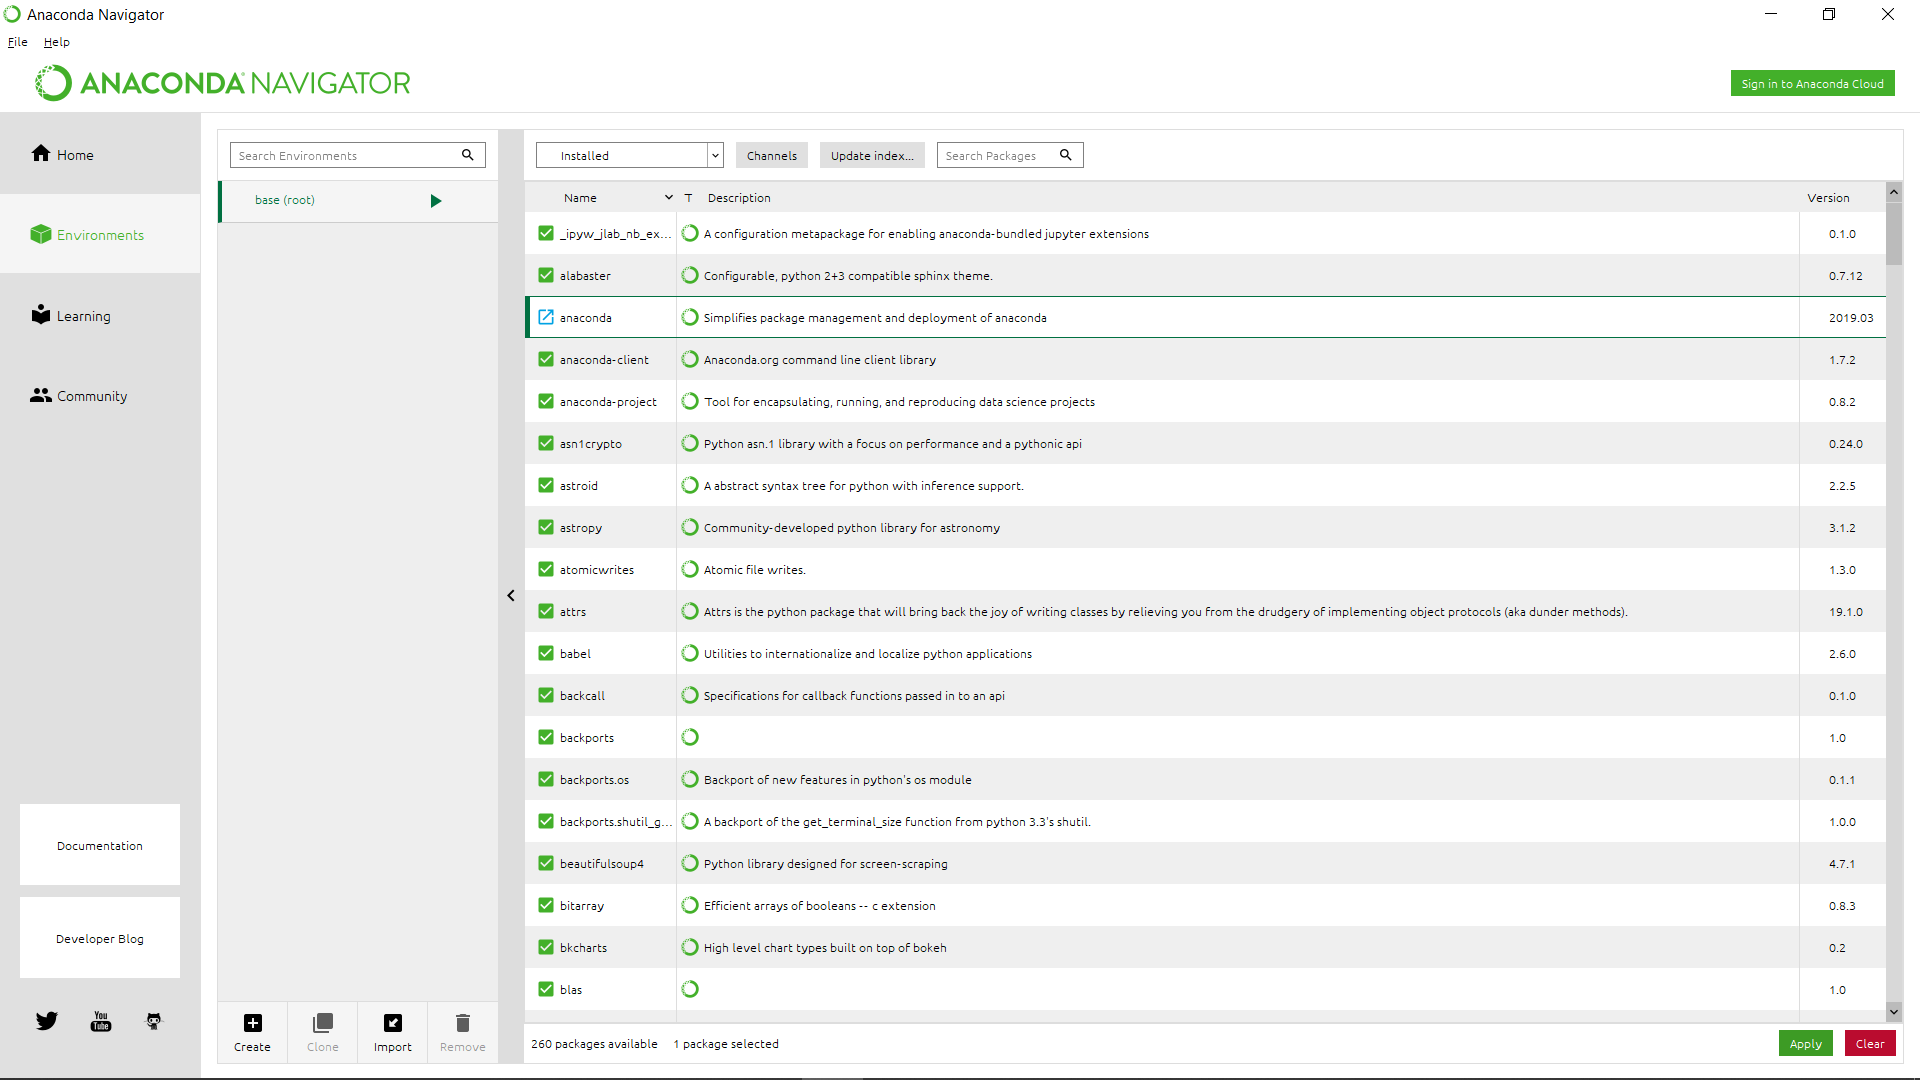
\includegraphics[scale=0.2]{figures/A7.png}
    \caption{Tahap kelima setting environment}
\end{figure}

    \begin{figure} [!htbp]
    \centering
    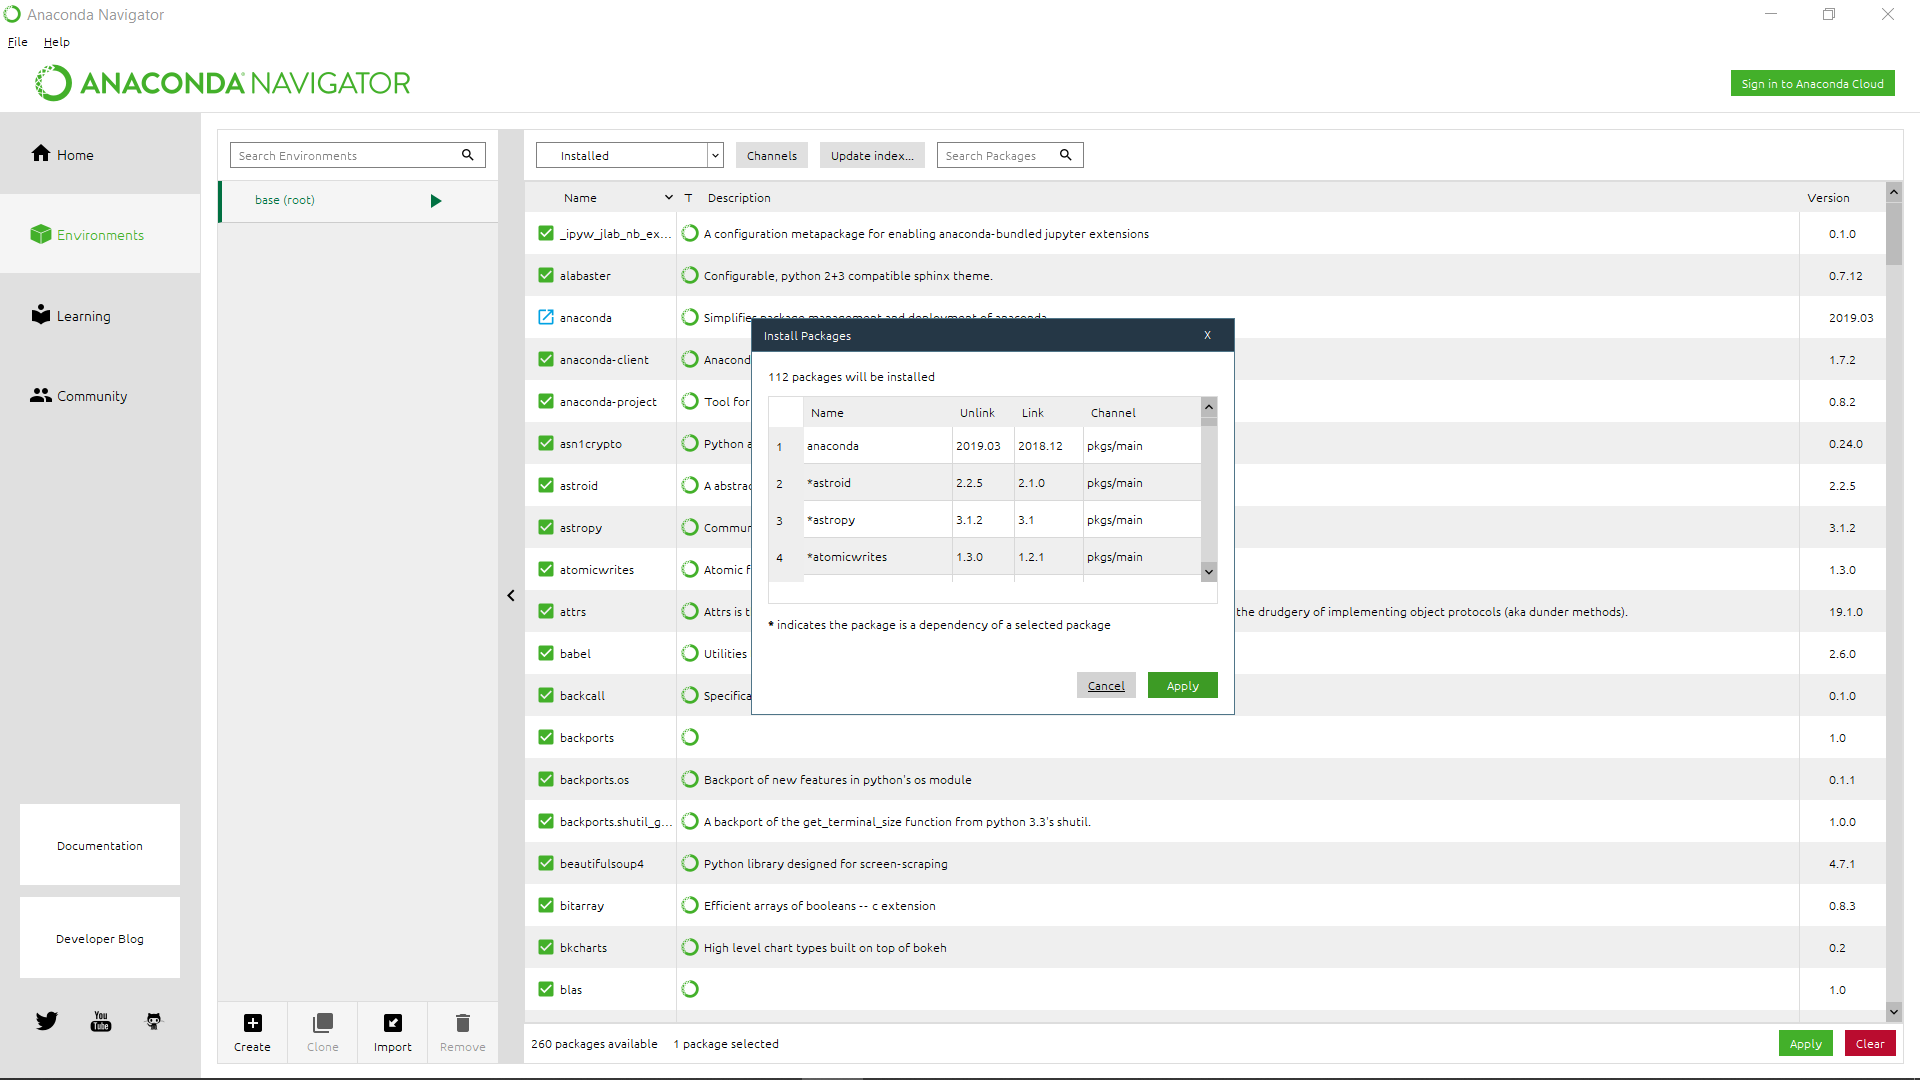
\includegraphics[scale=0.2]{figures/A8.png}
    \caption{Tahap keenam setting environment}
\end{figure}
\end{itemize}

\item Mencoba entrepreter/cli melakui terminal atau cmd windows
\begin{center}
    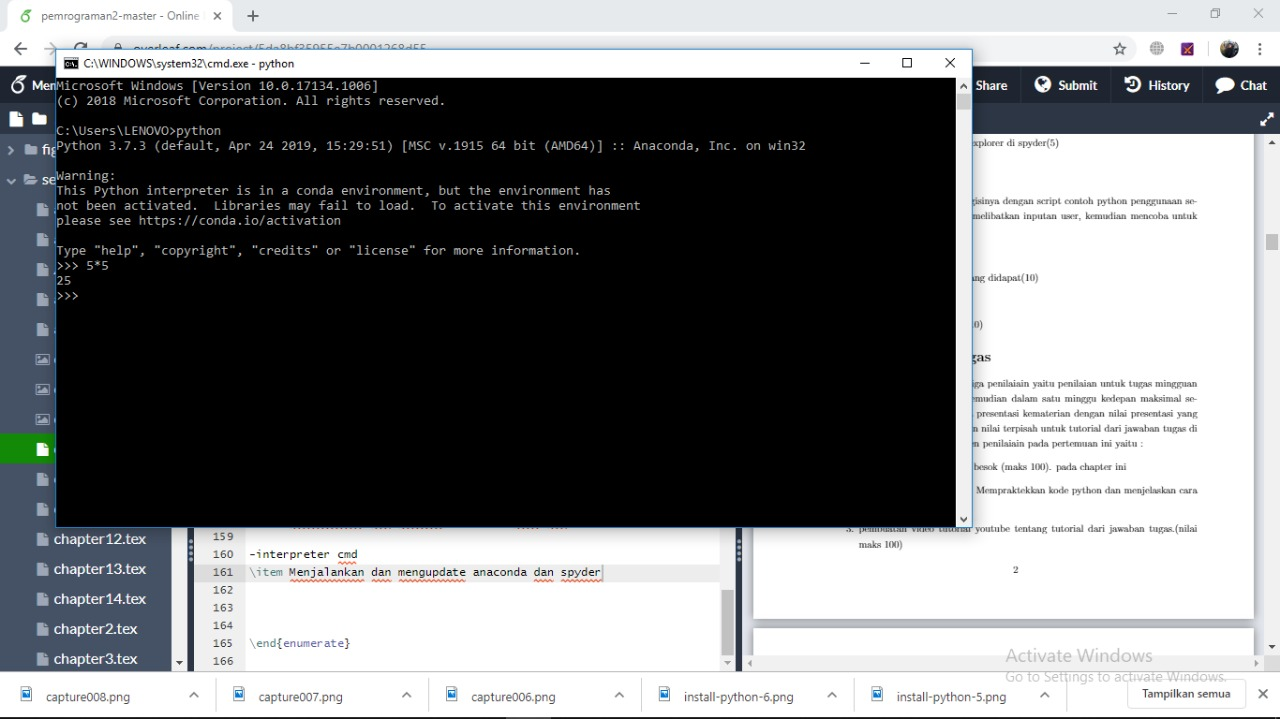
\includegraphics[width=10cm]{figures/Inter.jpeg}
\end{center}

\item 	Menjalankan Anaconda dan Spyder

\begin{itemize}
\item Install Anaconda di https://www.anaconda.com/distribution/
\item Jika sudah didownload, buka installer Anaconda
\begin{figure}[!htbp]
\centering
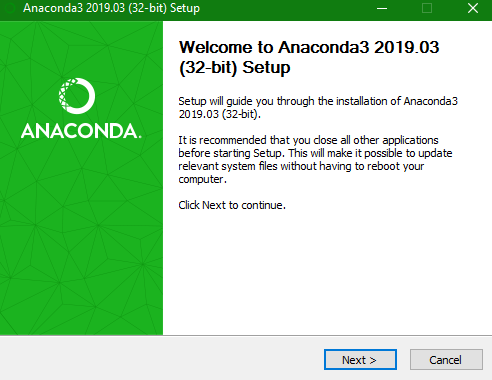
\includegraphics[scale=0.7]{figures/C1.png}
\caption{Tahap pertama penginstalan Anaconda}
\end{figure}
\item Klik Next.
\item Kemudian Pilih lokasi penyimpanan yang diinginkan
\begin{figure}[!htbp]
\centering
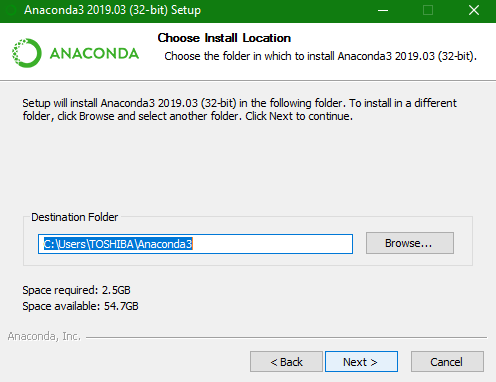
\includegraphics[scale=0.7]{figures/C2.png}
\caption{Tahap kedua penginstalan Anaconda}
\end{figure}
\item Lalu pilih Just Me(recommended) agar sesuai dengan komputer yang anda miliki
\begin{figure}[!htbp]
\centering
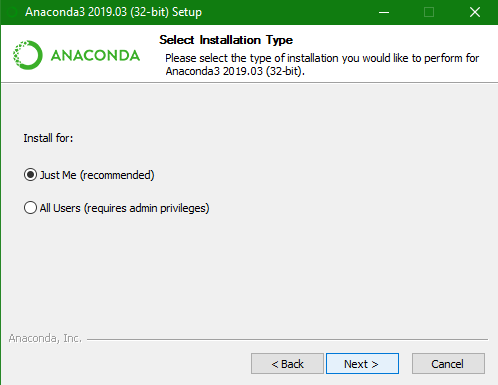
\includegraphics[scale=0.7]{figures/C3.png}
\caption{Tahap ketiga penginstalan Anaconda}
\end{figure}
\item Klik Next.
\item Kemudian ceklis Add Anaconda to my PATH
\begin{figure}[!htbp]
\centering
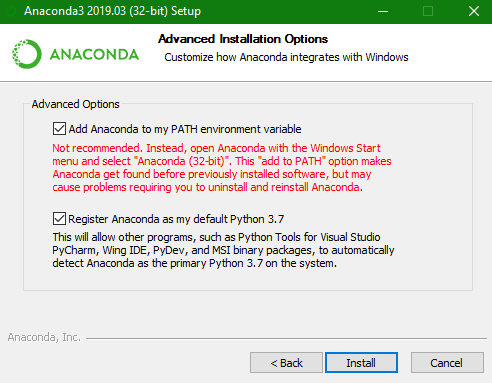
\includegraphics[scale=0.7]{figures/C4.png}
\caption{Tahap keempat penginstalan Anaconda}
\end{figure}
\item Lalu anda centang Add Anaconda to my Path environment variable, agar saat mengisntall selenium langsung ke path anaconda tidak ke aplikasi yang lain.
\item Jika sudah klik install, tunggu sampai selesai proses installasi selesai.
\begin{figure}[!htbp]
\centering
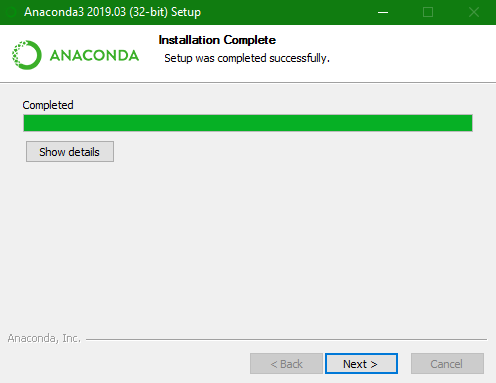
\includegraphics[scale=0.7]{figures/C5.png}
\caption{Tahap kelima penginstalan Anaconda}
\end{figure}
\item Klik Next.
\begin{figure}[!htbp]
\centering
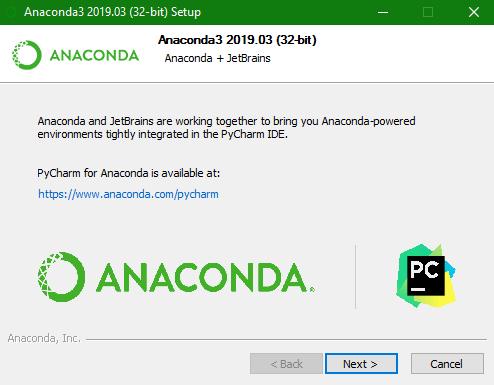
\includegraphics[scale=0.7]{figures/C6.png}
\caption{Tahap keenam penginstalan Anaconda}
\end{figure}
\item Klik Next.
\begin{figure}[!htbp]
\centering
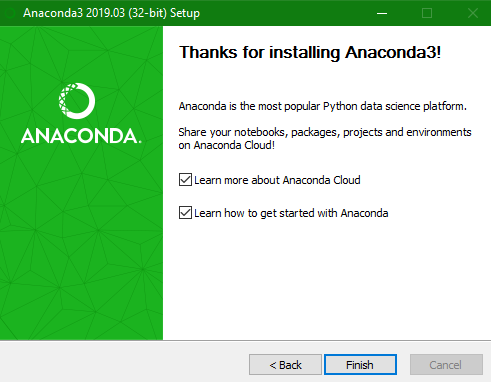
\includegraphics[scale=0.7]{figures/C7.png}
\caption{Tahap ketujuh penginstalan Anaconda}
\end{figure}
\item Jika sudah klik Finish
\end{itemize}

\item Cara menjalankan Script hello word di spyder
\begin{figure}[!htbp]
\centering
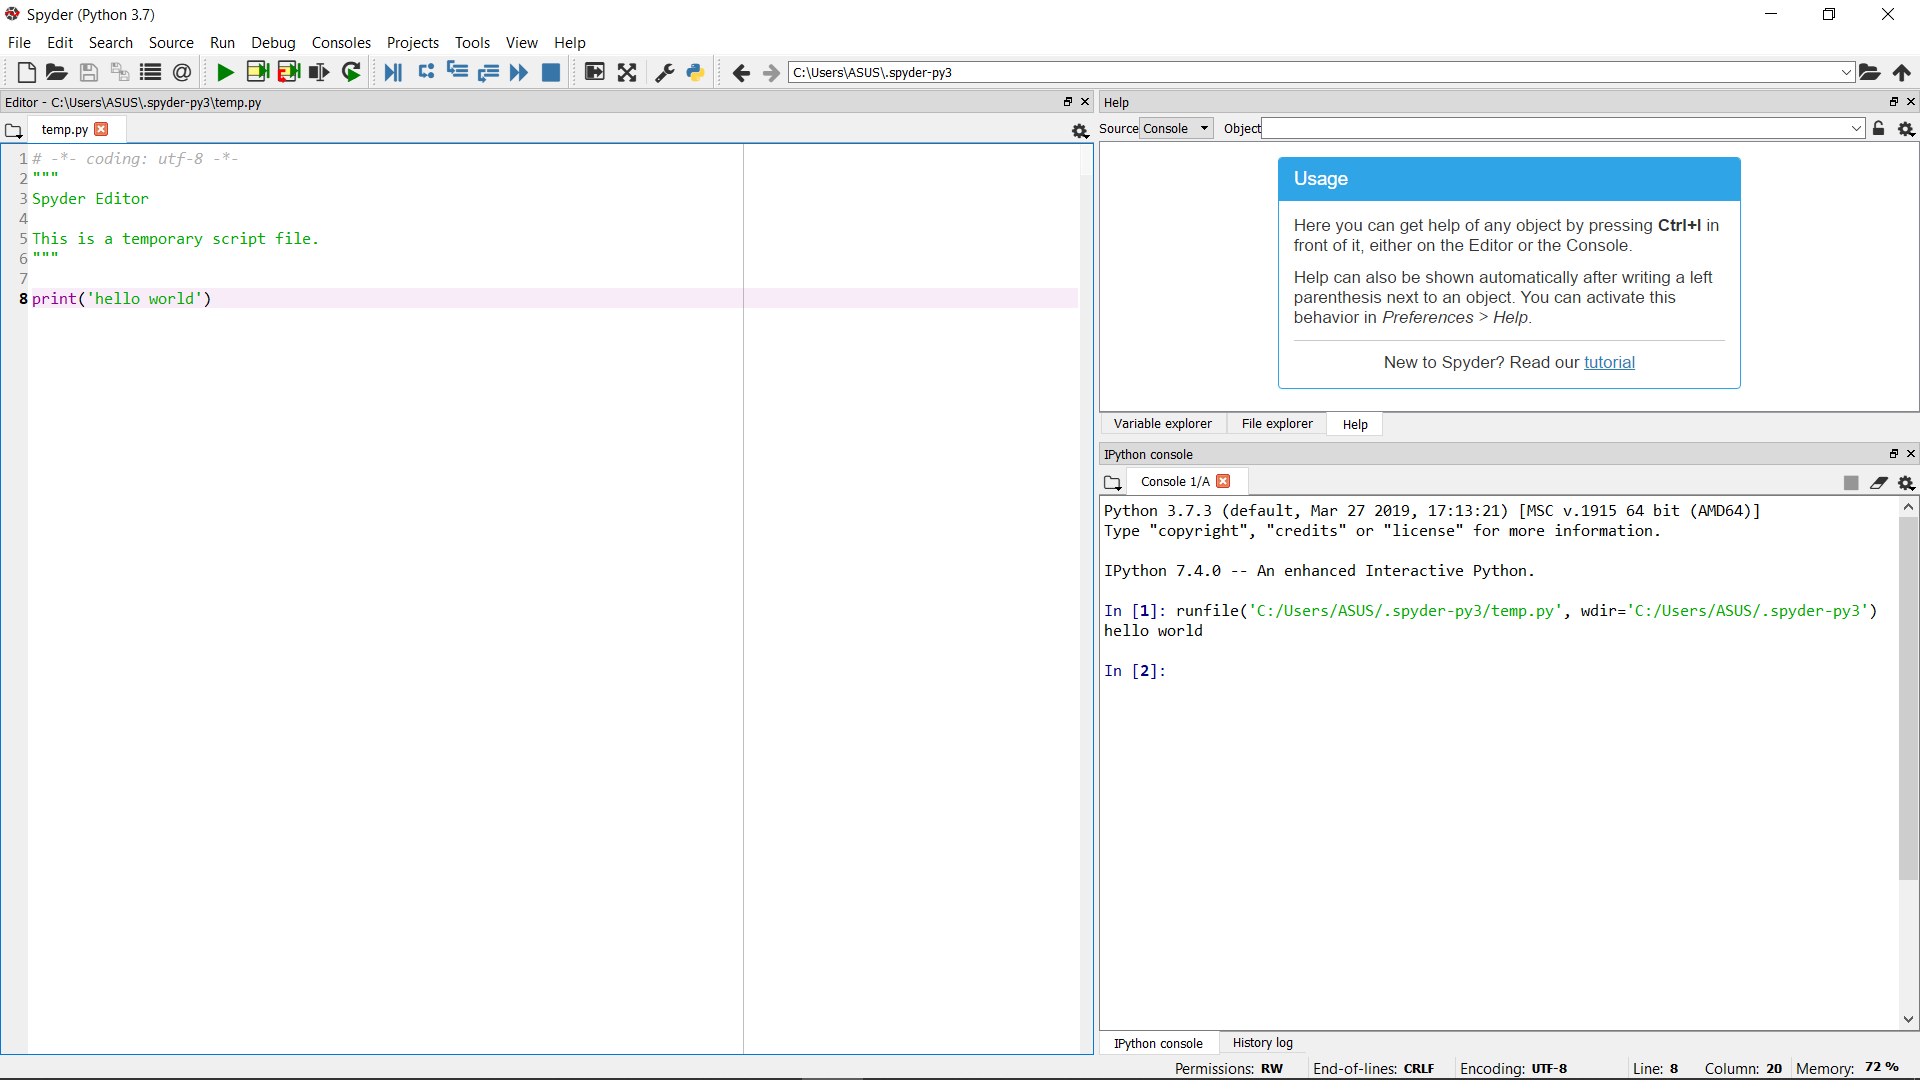
\includegraphics[scale=0.2]{figures/A2.png}
\caption{Menampilkan "Hello World"}
\end{figure}

\item Cara menjalankan Script otomatis login aplikasi akademik dengan library selenium dan inputan user
\begin{itemize}
\item Buka Spyder yang sudah di instal (Figure 1.22)
\begin{figure}[!htbp]
\centering
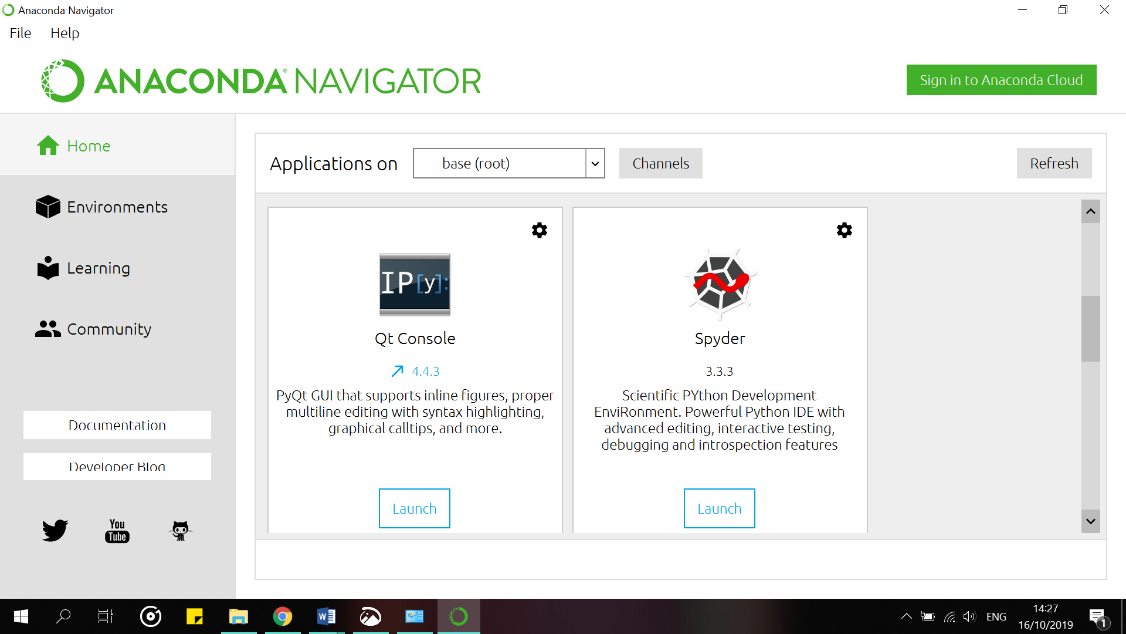
\includegraphics[scale=1]{figures/S1.png}
\caption{Tahap pertama menjalankan script otomatis}
\end{figure}
\item Kemudian ketik codingan berikut (Figure 1.23)
\item Run Codingan yang telah diketik.
\item Maka secara otomatis website siap.poltekpos.ac.id terbuka secara otomatis (Figure 1.24)
\begin{figure}[!htbp]
\centering
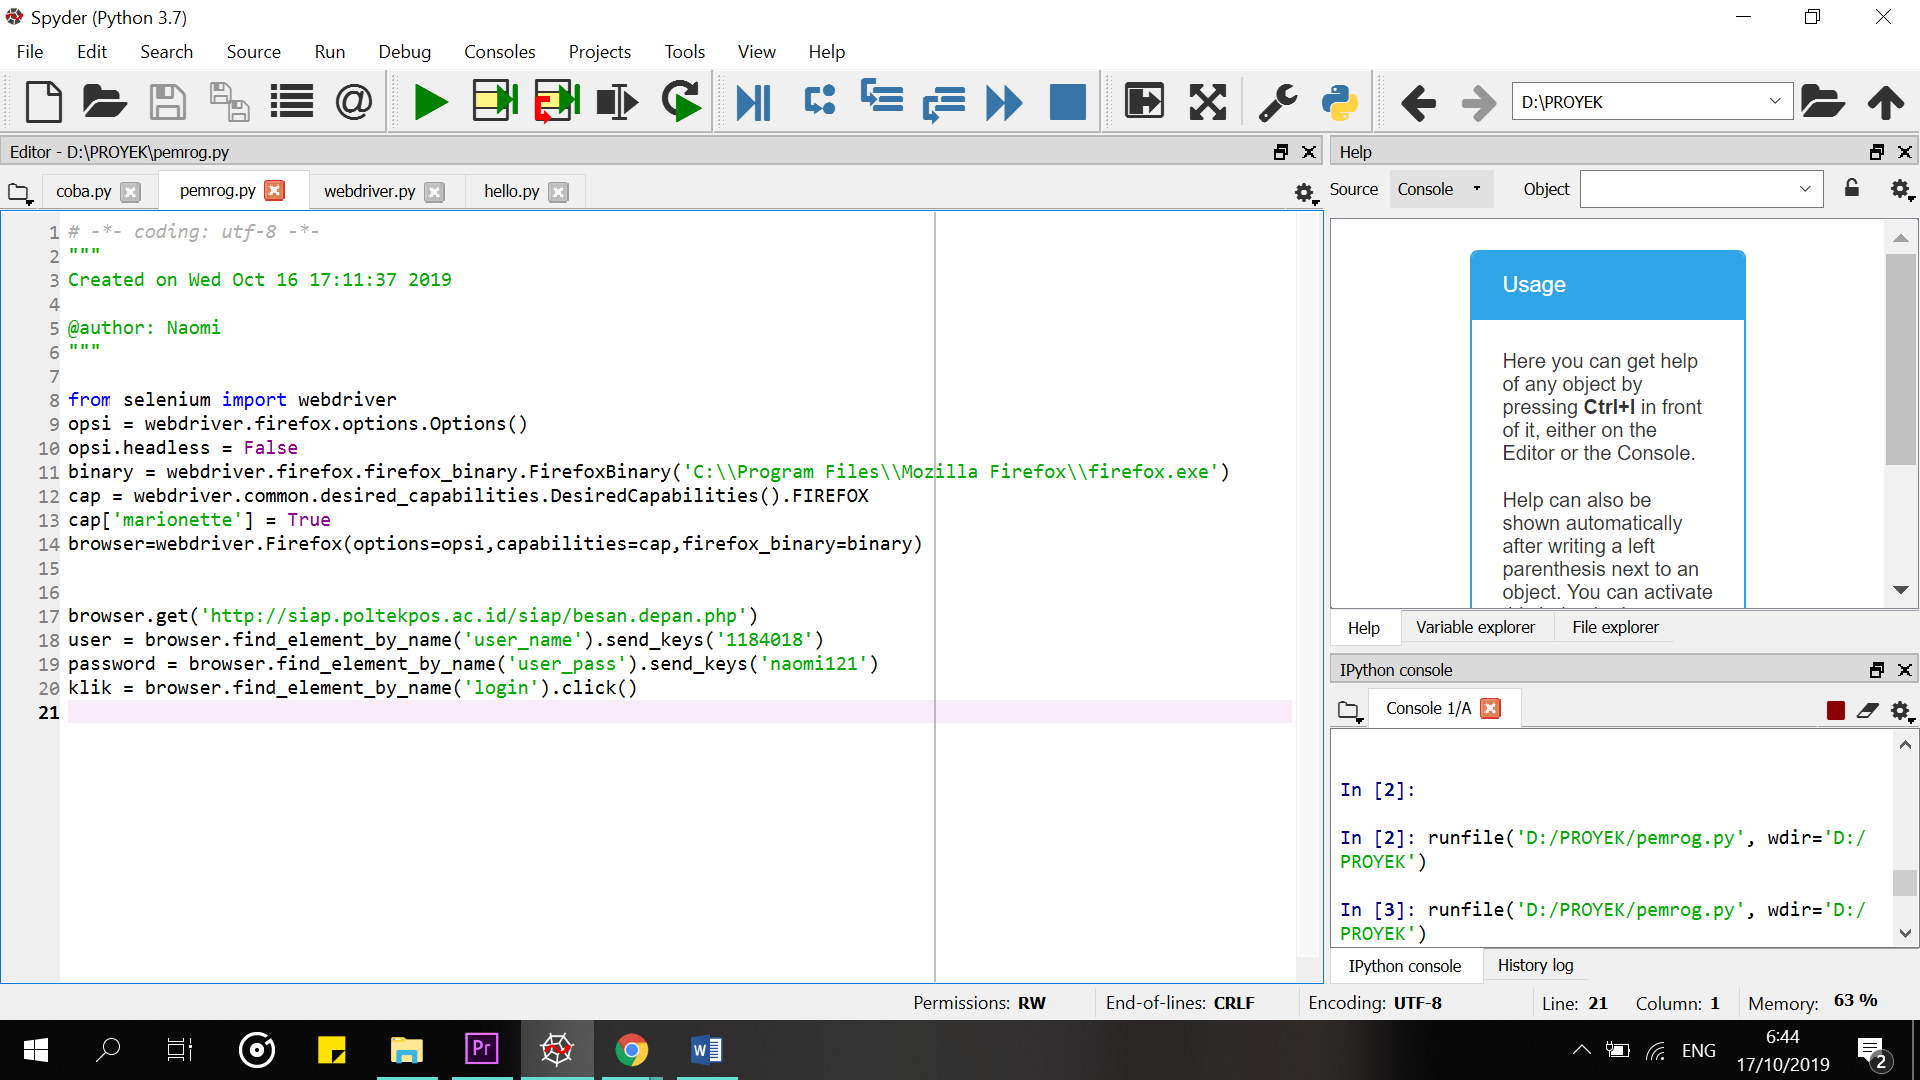
\includegraphics[scale=0.2]{figures/S4.png}
\caption{Tahap kedua menjalankan script otomatis}
\end{figure}
\begin{figure}[!htbp]
\centering
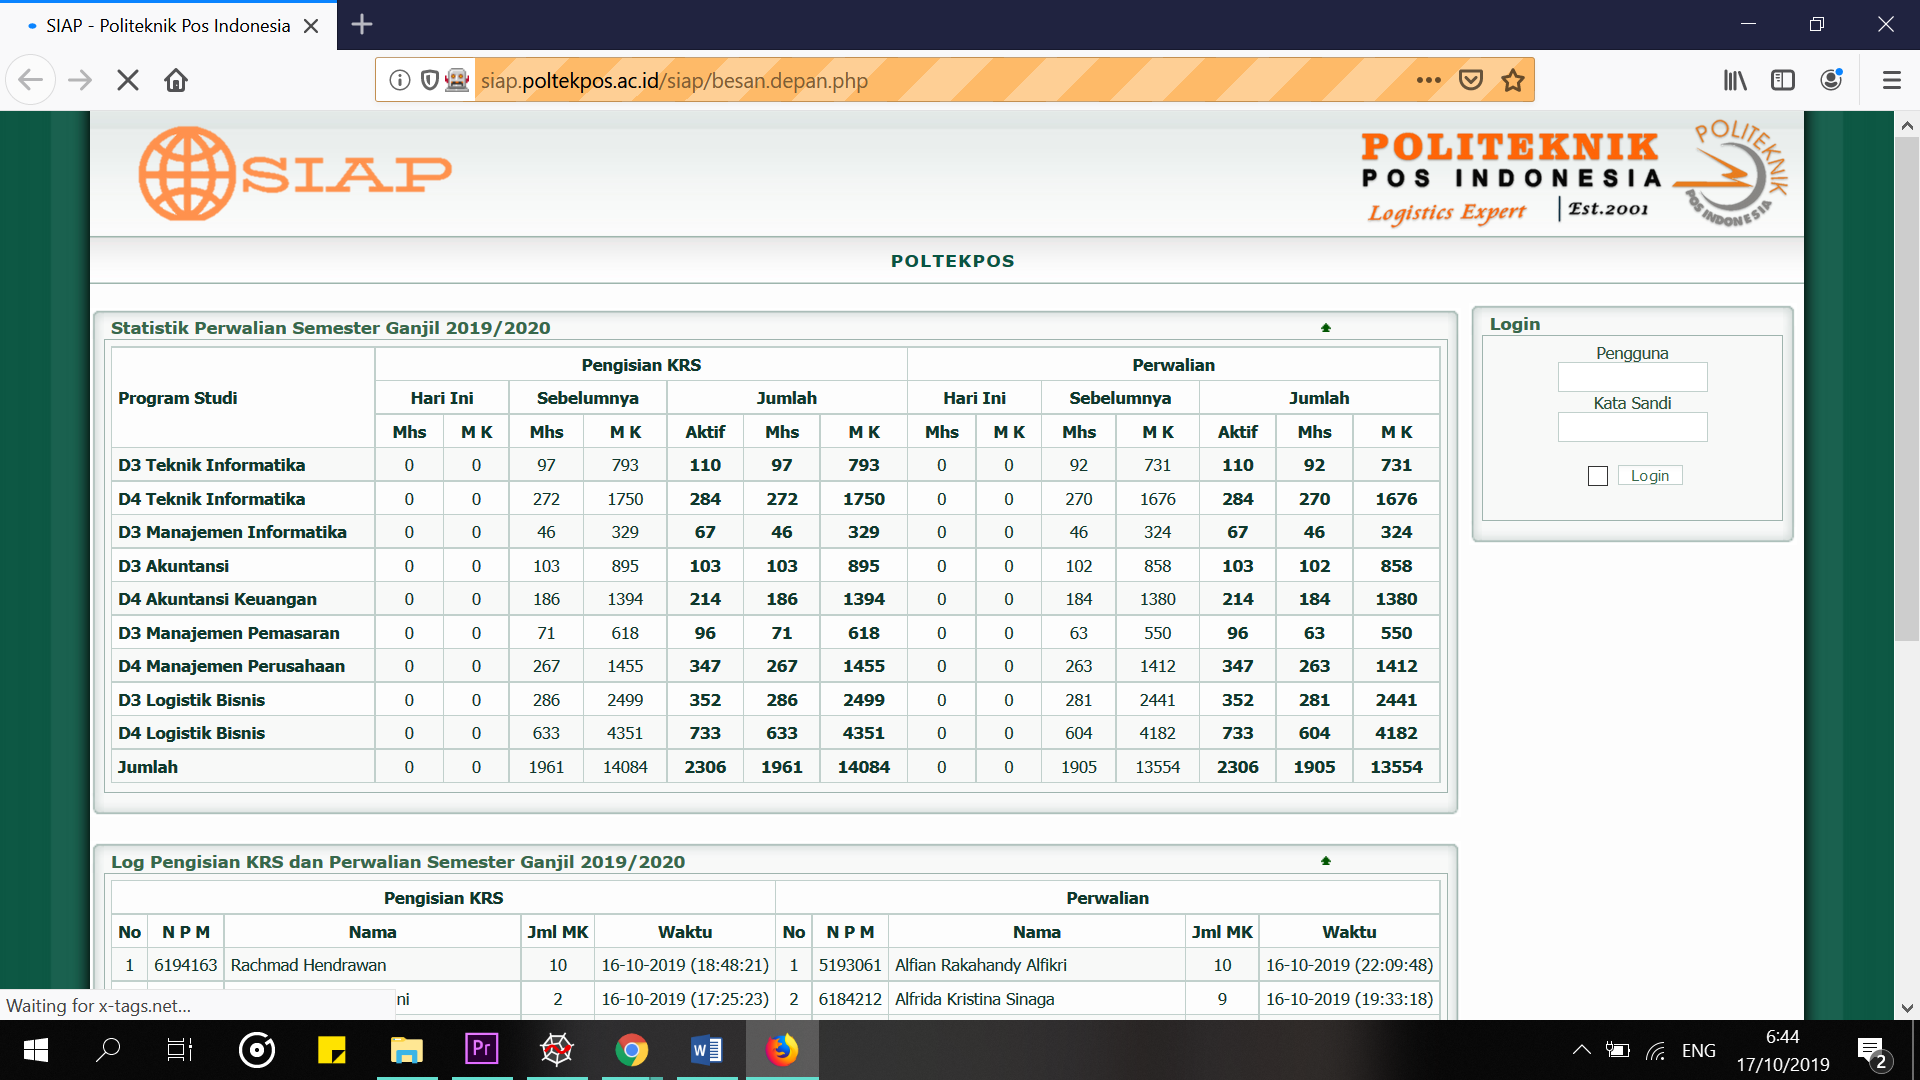
\includegraphics[scale=0.2]{figures/S5.png}
\caption{Tahap ketiga menjalankan script otomatis}
\end{figure}
\begin{figure}[!htbp]
\centering
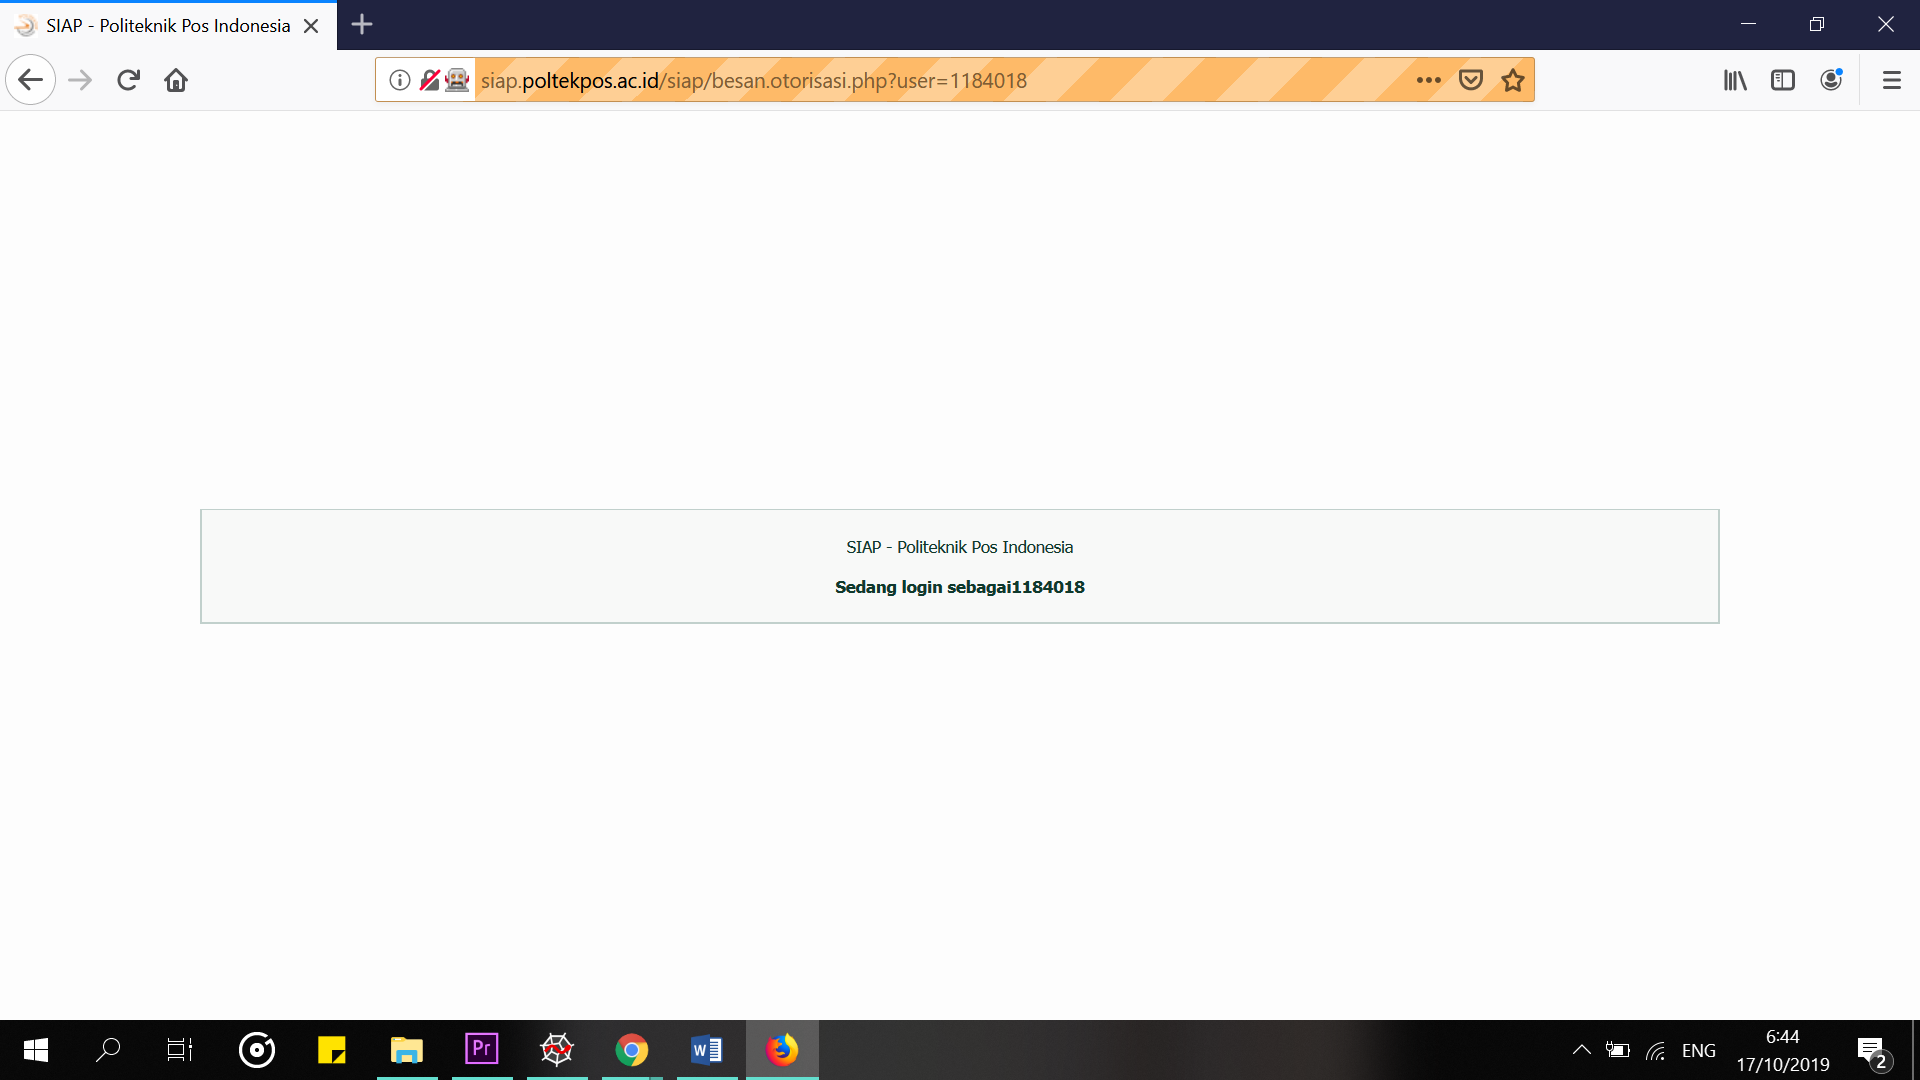
\includegraphics[scale=0.2]{figures/S6.png}
\caption{Tahap keempat menjalankan script otomatis}
\end{figure}
\end{itemize}

\item Cara pemakaian variable explorer di spyder (Figure 26)
\begin{figure}[!htbp]
\centering
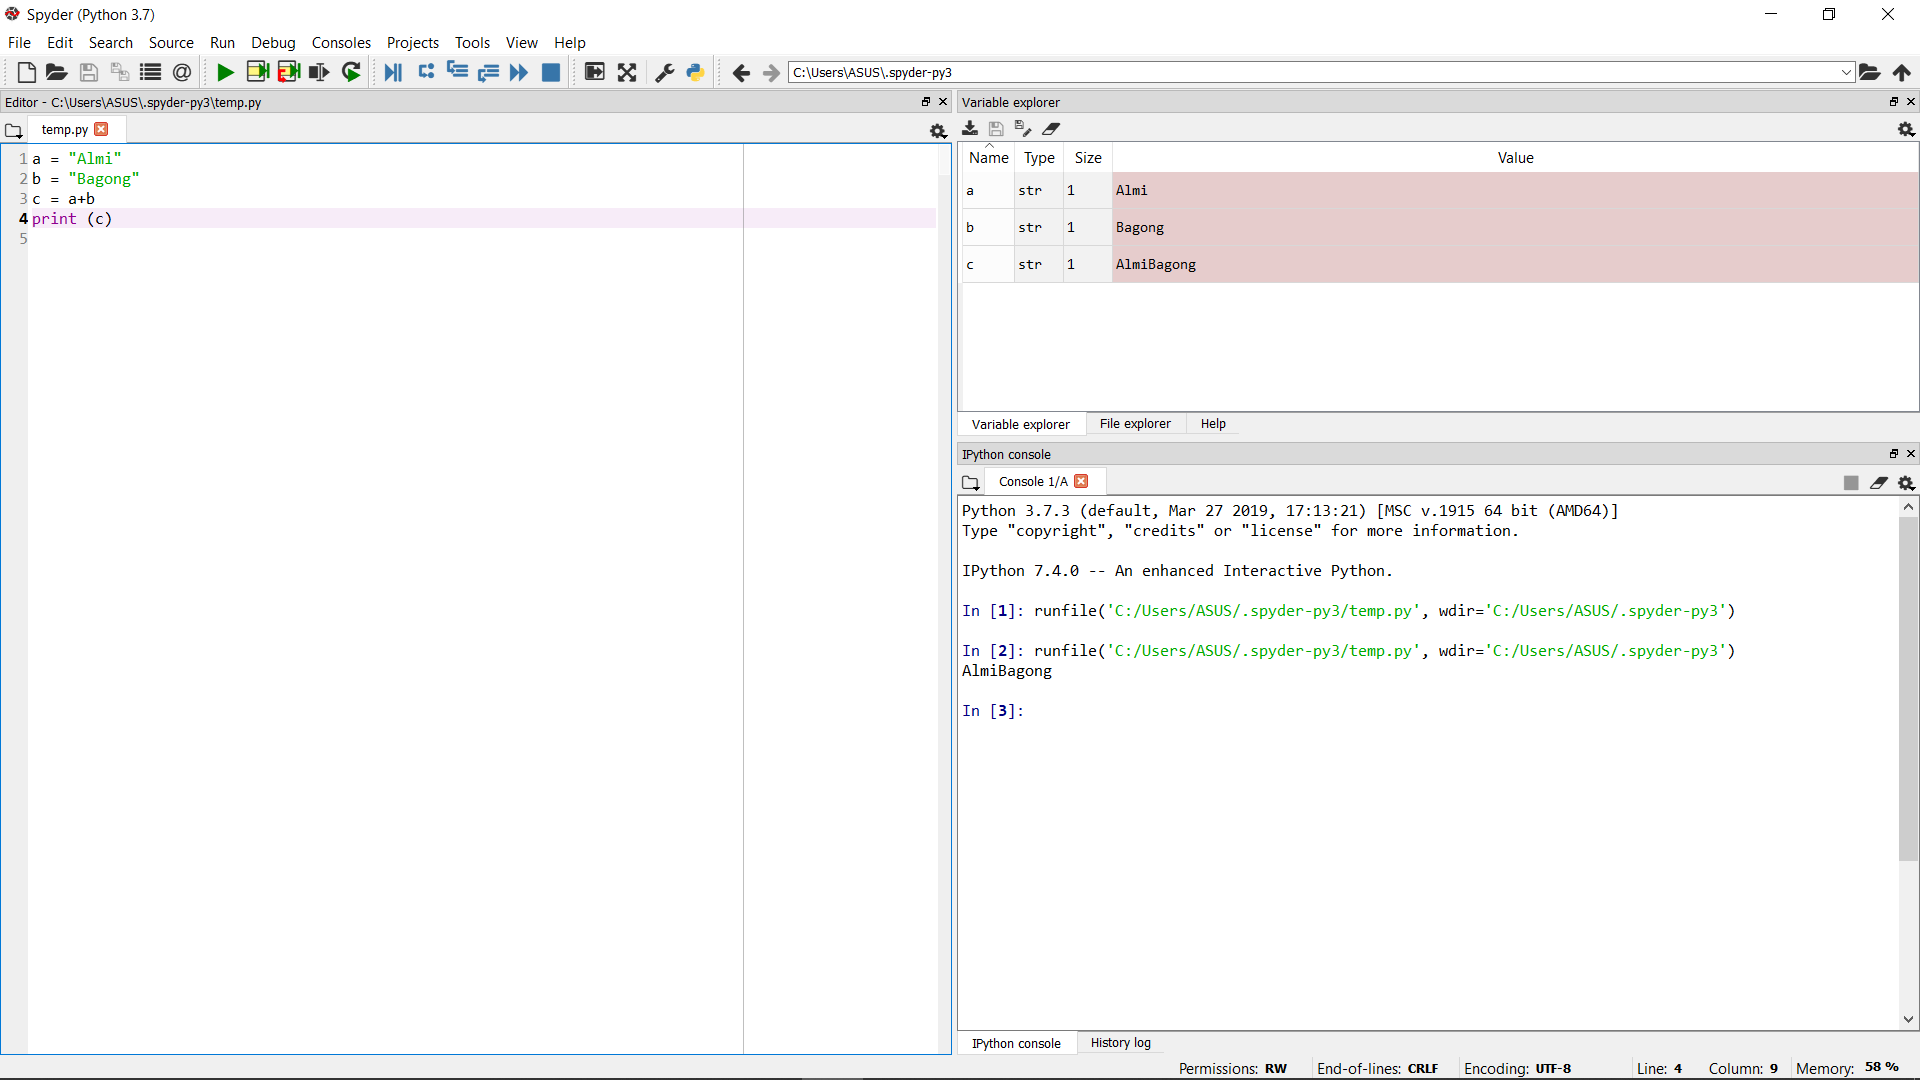
\includegraphics[scale=0.2]{figures/8.png}
\caption{Cara pemakaian variable explorer di spyder}
\end{figure}

\end{enumerate}